\documentclass[10pt]{article}
\usepackage{amsmath}
\usepackage{anysize}
\usepackage{amssymb}
\usepackage{graphicx}
\graphicspath{ {.} }
\title{COSC363 Assignment 1}
\author{Liam Pribis 81326653}
\date{29 April, 2020}
\marginsize{3em}{6em}{5em}{5em}

\begin{document}
\maketitle
    \section{Models}
    \subsection{Serpinski Tetrahedron}
    
    The serpinski tetrahdron is composed of many small tetrahedrons which are programmatically generated. Each tetrahdron is represented by a \verb|Tetra_t| struct, and a list of these is stored in a buffer. To draw the object, the buffer is iterated over and each tetrahedron is drawn individually. The model starts as a single large tetrahedron which is iteratively subdivided to create the final shape. During a subdivide operation, each tetrahedron is converted into four smaller tetrahedrons. Pressing 's' in the program will do this operation. To achieve the pulsating enlarging and reduction of tetrahedrons, each \verb|Tetra_t| has two sets of vertices. One set is directly inherited from the tetrahedron's parent, the other set is the one computed on subdivision. Each tetrahedron has the ability to linearly interpolate between these two sets of vertices. The amount of linear interpolation is controlled by a sine wave that acts over each tetrahedron based on its height in the structure, giving the vertical pulsing. Color is also assigned based on a tetrahedrons height in the structure. Since this model is completely procedurally generated, no sketches were used in it's construction.

    \subsection{Planets}
    The planets model is composed of a sun with two planets orbiting it. All objects are spinning on their vertical axis in some way. While there are only three planets, the program supports any number of planets each with custom orbit speeds, orbit radii, planet radii, and planet rotation speeds (three were chosen because I could not find suitable textures for any other planets). Each planet is drawn as a texture mapped cube. The on-axis rotation of each planet is done using \verb|glRotate|, while the orbits of planets are done using \verb|glTranslate| and sine/cosine.

    \subsection{Fire}
    The fire is a particle system comprised of upwards moving spheres. Each sphere moves upwards at a randomised speed. As it moves upwards, its color changes on a gradient from white to yellow to red to black. Each particle is represented by a \verb|Particle_t| struct, which holds all relevent information for each particle. On initialiization, a large buffer of particles is initialised with random locations, random speeds, and random max heights. Each update step, particles move upwards based on their speed. If they reach their max height, the particle starts over at the bottom of the particle system. This allows the same buffer of particles to be used without updating the buffer constantly.

    \subsection{Julia Set Surface}
    The julia set surface is a procedurally generated surface that moves based on a julia set to the fourth power, which gives a complex fractal surface that is rotationally symmetrical in four rotations. The surface also has procedurally generated normals, giving it shading. The surface is also procedurally colored based on a red to blue gradient. The color is derived from the height each point rises from the surface's origin. Due to varying input parameters, the surface moves in an unpredictable but continuous way. These parameters are generated from a number of sine and cosine waves added together. Higher frequency waves affect the inputs less than low frequency waves. This is similar to noise harmonics commonly used in procedural generation. The effect of these waves is a sporadic yet continuous varying of the surface.
\section{Extra features}
    \subsection{Generated surface}
    The julia set surface is generated per vertex in an iterative fashion. For each vertex, an algorithm is applied to determine the value (which then will determine the height of the vertex off of the surface and the vertex's color). The algorithm is usually implemented using complex numbers, but in this case each number was separated into its real and immaginary components (to get rid of a dependency on the C complex numbers library).

    For each vertex, a complex number $z$ is created based on the normalised x and y position of the vertex in the surface. Another compelx number $c$ is constant for each frame of the animating surface (generation of $c$ discussed below). The equation $z = z^4 + c$ is applied over and over until $z$ escapes a circle of predetermined raduis. Normally, the number of iterations is used to determine the value of a vertex, but this was not used because it yielded a very "spiky" surface which was not very visually pleasing (due to the large and rapid gradient of the iteration count over the surface).

    Intstead the value of each vertex is a real number initialised to $e^{-\sqrt{z}}$. Each iteration, the value is updated using $value = value + e^{-\sqrt{z}}$. Since a small magnitude is being added each iteration, rather than an integer, the gradient of the surface is much smoother. The exponentiation of a negative value ensures that even with a large number of iterations, the value will stay within a defined range (due to the diminishing returns of $e^{-x}$).

    Note that the above equations are not the ones actually used in the program. Instead of complex $z$, $zx$ and $zy$ are used, which represent the real and complex parts of $z$. The same is done with $c$. Instead of $z = z^4+c$ the following equations are used, which are simple the expansion of $(zx+zy i)^4+(cx+cy i)$.
    $$zx = zx * zx * zx * zx + zy * zy * zy * zy - 6 * zx * zx * zy * zy + cx$$
    $$zy = 4 * zx * zx * zx * zy - 4 * zx * zy * zy * zy + cy$$

    The values of $cx$ and $cy$ are given by a series of sine and cosing waves. Higher harmonics of waves have smaller amplitudes, giving a pseudorandom but continuous walk around the xy plane. Since the $cx$ and $cy$ completely determine the shape of any given julia set, a random walk with continuous $cx$ and $cy$ will give a continuous julia set with no "jumps".
    \subsection{Skybox}
    The skybox is a cube with inverted normals that is texture mapped to 6 desert textures, one for each face. The cube is drawn and then scaled to 500x500x500.
    \subsection{Particle system}
    The particle system is made using a large number of independent objects. Each object is a struct and is updated individually. Each particle has an $x, z$ location, a speed and a height limit initialised randomly at the start. Each parameter has a different range of random numbers that can be assigned to it. When a particle is updated, it adds it's speed (plus a global speed control parameter) to its y height. If the particle reaches is maximum height, it reset's its height back to zero.

    The ratio of the particle's height to maximum height is used to determine the color. This is done instead of simply using the particle's height because it gives a more random gradient of fire (due to randomised maximum heights), instead of each particle changing color exactly at the same time as the particles next to it. The ratio of a particles height to its maximum height can be thought of as the particles "age" (which will always go from zero to one and reset to zero). To generate a particles color, the particle's age is split into three ranges, 0-0.25, 0.25-0.5, and 0.5-1. Each range has it's own color gradient:  first from white to yellow, then from yellow to red, then from red to black. Since neighboring ranges have the same colors, the color transition is always smooth.
    
    \section{Controls}
    \begin{itemize}
        \item Left and right arrow keys change the angle of the camera.
        \item Up and down arrow keys move the camera forward and backward.
        \item 'S' subdivides the serpinski tetrahedron.
    \end{itemize}
    Note camera controls do not operate on "keydown" rising edge events, they operate on whether a key is held down in the current moment.

    \section{Building the Project}
    No build system helper is used for this project, only a bash script and gcc. The script \verb|build| handles this. It simply runs gcc on every .c file in \verb|/src/| and produces a corresponding .o in \verb|/out/|, and then links all of these files with \verb|main.o| and opengl, producing the executable \verb|main|.
    \subsection{Usage}
    \begin{itemize}
        \item \verb|./build clean| - remove everything in the output directory.
        \item \verb|./build build| - compile and link, but do not run. The executable is \verb|/out/main|.
        \item \verb|./build run| - clean, then compile, then run the executable.
    \end{itemize}
    \section{References}
    \begin{itemize}
        \item Julia set algorithm https://mathworld.wolfram.com/JuliaSet.html
        \item Earth texture https://www.cleanpng.com/png-earth-texture-mapping-sphere-cube-mapping-1618609/
        \item Mars texture https://source.opennews.org/articles/how-we-made-rewind-red-planet/
        \item Sun texture https://www.solarsystemscope.com/textures/
        \item Brick texture https://commons.wikimedia.org/wiki/File:Red-brick-wall-texture-clean.jpg
    \end{itemize}

    \section{Screenshots}

    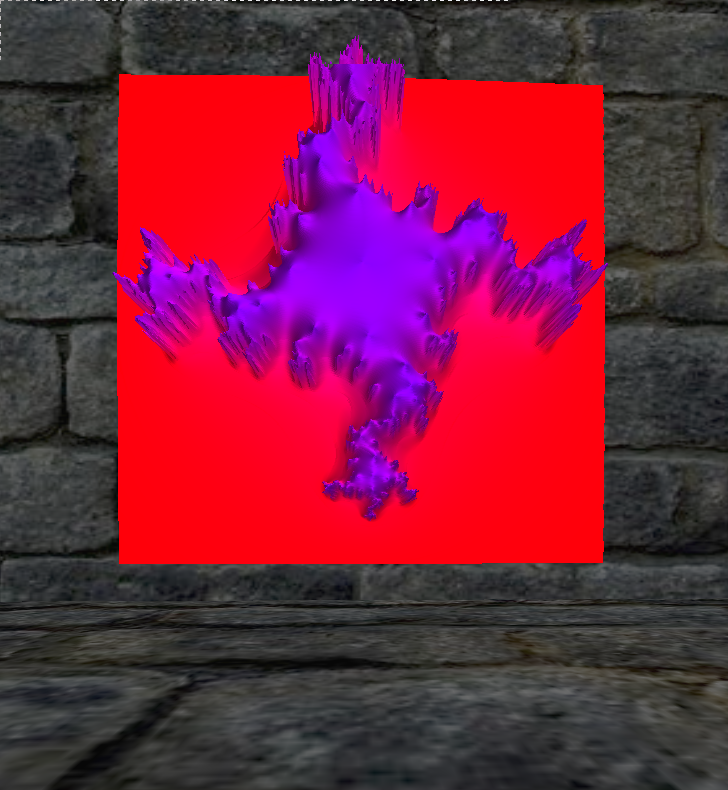
\includegraphics[scale=0.2]{rr1.png}
    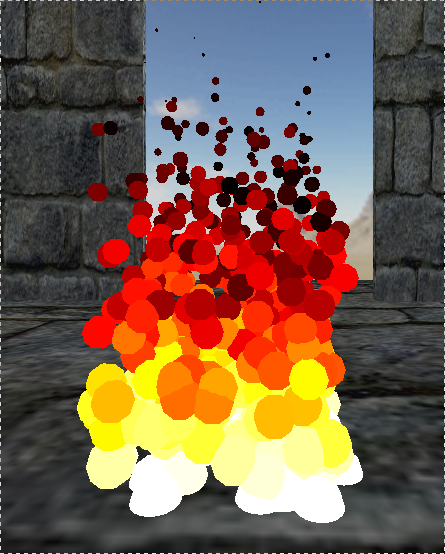
\includegraphics[scale=0.3]{rr2.png}
    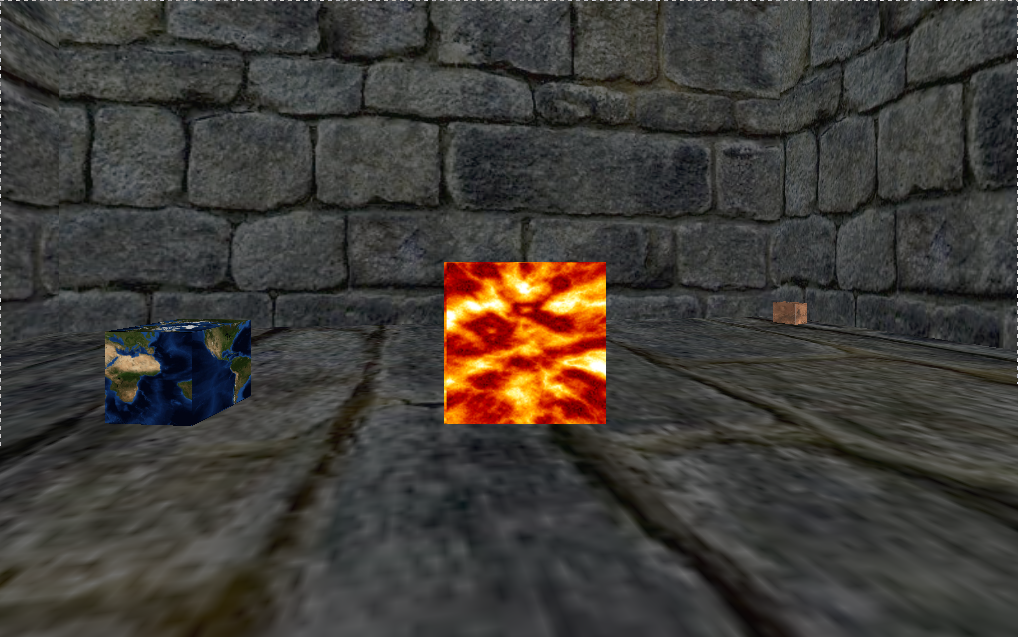
\includegraphics[scale=0.3]{rr3.png}
    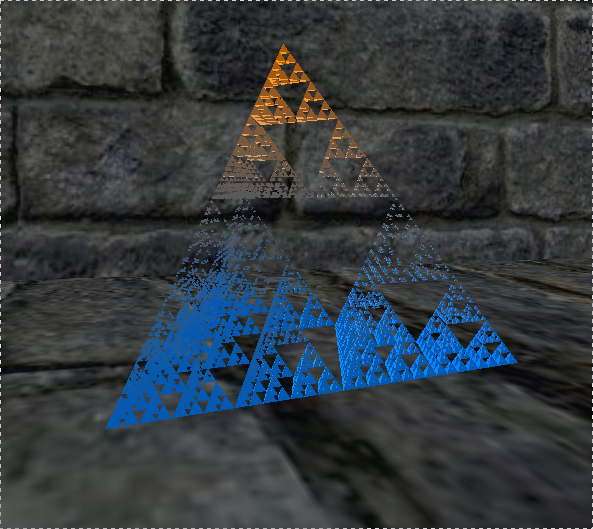
\includegraphics[scale=0.3]{rr4.png}
\end{document}